
\chap{结论}
If you have reached this chapter, having read the previous seven chapters, then there is a good chance that you have understood what a quaternion is, and how it is used to rotate vectors about an arbitrary axis. I deliberately played down the four-dimensional side of quaternions, as this feature is not relevant to understanding what they are, and how they are manipulated at an introductory level. You should now be in a position to code up the operations and discover what benefits quaternions bring to the stage of rotations. You should also be in a position to tackle more advanced texts and discover other applications.

Very rarely, has any mathematician invented something that has taken the world completely by surprise. For as we have seen with the invention of quaternions, Gauss had played around with quadruples, but was too nervous to tell anyone. Similarly, Grassmann had also been working on his own vector algebra and had written up his ideas in two books, but his style of writing was too obscure, even for mathematicians to understand! Rodrigues has been described as a 'recreational' mathematician, and perhaps just for the fun of it, decided to analyse the algebra of rotations. In so doing, he discovered a half-angle solution identical to that of the quaternion product, three years ahead of Hamilton. But in the end, it was left to Hamilton to successfully generalise complex numbers to a higher dimension. It took him over a decade to discover the final solution, and in spite of being a genius, he was unaware that a triple could not be the answer. Fortunately, his tenacity and mathematical brilliance shone through and won the day.

Although Hamilton thought that quaternions would become an important mathematical tool for a wide range of scientific applications, they were ignored in favour of the vector algebra described by Gibbs. Hamilton must have been disappointed that quaternion algebra did not become the preferred vectorial system, but he should have been extremely proud to have been responsible for the event that gave us today's vector algebra.

It is interesting that the computer age, and especially the subject of computer graphics, has provided a useful application for quaternions. Perhaps we can at last forget about Euler rotations and work with a mathematical tool that is intuitive, easy to use and efficient-quaternions!

\section{Appendix
Eigenvectors and Eigenvalues}
This appendix shows how to compute the eigenvector of a rotation matrix.

Given a square matrix $\mathbf{A}$, a non-zero vector $\mathbf{v}$ is an eigenvector, and $\lambda$ is the corresponding eigenvalue if

$$
\mathbf{A v}=\lambda \mathbf{v}, \quad \lambda \in \mathbb{R} .
$$

The German word eigen means characteristic, own, latent or special, and eigenvector means a special vector associated with a transform. The equation that determines the existence of any eigenvectors is called the characteristic equation of a square matrix, and is given by

$$
\operatorname{det}(\mathbf{A}-\lambda \mathbf{I})=0 .
$$

To illustrate how we solve the characteristic equation (A.1) we start with three simultaneous equations:

$$
\begin{aligned}
3 x+z & =0 \\
-x+3 y+3 z & =0 \\
x+3 z & =0
\end{aligned}
$$

which can be represented in matrix form as

$$
\left[\begin{array}{ccc}
3 & 0 & 1 \\
-1 & 3 & 3 \\
1 & 0 & 3
\end{array}\right]\left[\begin{array}{l}
x \\
y \\
z
\end{array}\right]=\left[\begin{array}{l}
0 \\
0 \\
0
\end{array}\right]
$$

If

$$
\mathbf{A}=\left[\begin{array}{ccc}
3 & 0 & 1 \\
-1 & 3 & 3 \\
1 & 0 & 3
\end{array}\right]
$$

its characteristic equation is

$$
\left|\begin{array}{ccc}
3-\lambda & 0 & 1 \\
-1 & 3-\lambda & 3 \\
1 & 0 & 3-\lambda
\end{array}\right|=0
$$

Expanding the determinant using the top row we have

$$
\begin{aligned}
(3-\lambda)\left|\begin{array}{cc}
3-\lambda & 3 \\
0 & 3-\lambda
\end{array}\right|-0+\left|\begin{array}{cc}
-1 & 3-\lambda \\
1 & 0
\end{array}\right| & =0 \\
(3-\lambda)(3-\lambda)^{2}-(3-\lambda) & =0 \\
(3-\lambda)\left[(3-\lambda)^{2}-1\right] & =0 \\
(3-\lambda)\left(\lambda^{2}-6 \lambda+8\right) & =0 \\
(3-\lambda)(\lambda-4)(\lambda-2) & =0
\end{aligned}
$$

which has solutions $\lambda=2,3,4$. Let's substitute these values of $\lambda$ in the original equations to reveal the eigenvectors.

\begin{center}
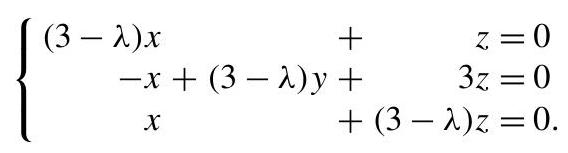
\includegraphics[max width=\textwidth]{2023_01_16_a848224efad29cd66460g-149}
\end{center}

With $\lambda=2$ we have $z=-x$ from the 1 st equation. Substituting this in the 2 nd equation we have $y=4 x$, which permits us to state that the associated eigenvector is of the form $\left[\begin{array}{lll}k & 4 k & -k\end{array}\right]^{\mathrm{T}}$.

With $\lambda=3$ we have $z=0$ from the 1 st equation, and $x=0$ from the 3rd equation, which permits us to state that the associated eigenvector is of the form $\left[\begin{array}{lll}0 & k & 0\end{array}\right]^{\mathrm{T}}$.

With $\lambda=4$ we have $z=x$ from the 1 st equation. Substituting this in the 2 nd equation we have $y=2 x$, which permits us to state that the associated eigenvector is of the form $\left[\begin{array}{lll}k & 2 k & k\end{array}\right]^{\mathrm{T}}$.

Therefore, the eigenvectors and eigenvalues are

$$
\begin{array}{rrr}
{\left[\begin{array}{rrr}
k & 4 k & -k
\end{array}\right]^{\mathrm{T}}} & \lambda=2 \\
{\left[\begin{array}{lll}
0 & k & 0
\end{array}\right]^{\mathrm{T}}} & \lambda=3 \\
{\left[\begin{array}{lll}
k & 2 k & k
\end{array}\right]^{\mathrm{T}}} & \lambda=4
\end{array}
$$

where $k \neq 0$.

The major problem with this technique is that it requires careful analysis to untangle the eigenvector, and ideally, we require a deterministic algorithm to reveal the result, which is covered next.

We begin with the fact that a rotation matrix always has a real eigenvalue $\lambda=1$, which permits us to write

$$
\begin{aligned}
\mathbf{A} \mathbf{v} & =\lambda \mathbf{v} \\
\mathbf{A v} & =\lambda \mathbf{I} \mathbf{v}=\mathbf{I} \mathbf{v} \\
(\mathbf{A}-\mathbf{I}) \mathbf{v} & =\mathbf{0}
\end{aligned}
$$

therefore,

$$
\left[\begin{array}{ccc}
\left(a_{11}-1\right) & a_{12} & a_{13} \\
a_{21} & \left(a_{22}-1\right) & a_{23} \\
a_{31} & a_{32} & \left(a_{33}-1\right)
\end{array}\right]\left[\begin{array}{l}
x_{v} \\
y_{v} \\
z_{v}
\end{array}\right]=\left[\begin{array}{l}
0 \\
0 \\
0
\end{array}\right]
$$

Expanding (A.2) we have

$$
\begin{aligned}
& \left(a_{11}-1\right) x_{v}+a_{12} y_{v}+a_{13} z_{v}=0 \\
& a_{21} x_{v}+\left(a_{22}-1\right) y_{v}+a_{23} z_{v}=0 \\
& a_{31} x_{v}+a_{32} y_{v}+\left(a_{33}-1\right) z_{v}=0 .
\end{aligned}
$$

There exists a trivial solution where $x_{v}=y_{v}=z_{v}=0$, but to discover something more useful we can relax any one of the $v$ terms which gives us three equations in two unknowns. Let's make $x_{v}=0$ :

$$
\begin{aligned}
a_{12} y_{v}+a_{13} z_{v} & =-\left(a_{11}-1\right) \\
\left(a_{22}-1\right) y_{v}+a_{23} z_{v} & =-a_{21} \\
a_{32} y_{v}+\left(a_{33}-1\right) z_{v} & =-a_{31} .
\end{aligned}
$$

We are now faced with choosing a pair of equations to isolate $y_{v}$ and $z_{v}$. In fact, we have to consider all three pairings because it is possible that a future rotation matrix will contain a column with two zero elements, which could conflict with any pairing we make at this stage.

Let's begin by choosing (A.3) and (A.4). The solution employs the following strategy: Given the following matrix equation

$$
\left[\begin{array}{ll}
a_{1} & b_{1} \\
a_{2} & b_{2}
\end{array}\right]\left[\begin{array}{l}
x \\
y
\end{array}\right]=\left[\begin{array}{l}
c_{1} \\
c_{2}
\end{array}\right]
$$

then

$$
\frac{x}{\left|\begin{array}{ll}
c_{1} & b_{1} \\
c_{2} & b_{2}
\end{array}\right|}=\frac{y}{\left|\begin{array}{ll}
a_{1} & c_{1} \\
a_{2} & c_{2}
\end{array}\right|}=\frac{1}{\left|\begin{array}{ll}
a_{1} & b_{1} \\
a_{2} & b_{2}
\end{array}\right|} .
$$

Therefore, using the 1 st and 2 nd equations (A.3) and (A.4) we have

$$
\begin{aligned}
& x_{v}=a_{12} a_{23}-a_{13}\left(a_{22}-1\right) \\
& y_{v}=a_{13} a_{21}-a_{23}\left(a_{11}-1\right) \\
& z_{v}=\left(a_{11}-1\right)\left(a_{22}-1\right)-a_{12} a_{21} .
\end{aligned}
$$

Similarly, using the 1st and 3rd equations (A.3) and (A.5) we have

$$
\begin{aligned}
& x_{v}=a_{12}\left(a_{33}-1\right)-a_{13} a_{32} \\
& y_{v}=a_{13} a_{31}-\left(a_{11}-1\right)\left(a_{33}-1\right) \\
& z_{v}=a_{32}\left(a_{11}-1\right)-a_{12} a_{31}
\end{aligned}
$$

and using the 2nd and 3rd equations (A.4) and (A.5) we have

\begin{center}
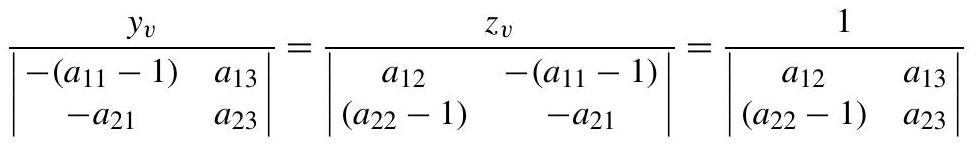
\includegraphics[max width=\textwidth]{2023_01_16_a848224efad29cd66460g-150}
\end{center}

$$
\begin{aligned}
& x_{v}=\left(a_{22}-1\right)\left(a_{33}-1\right)-a_{23} a_{32} \\
& y_{v}=a_{23} a_{31}-a_{21}\left(a_{33}-1\right) \\
& z_{v}=a_{21} a_{32}-a_{31}\left(a_{22}-1\right) .
\end{aligned}
$$

Now we have nine equations to cope with any eventuality. In fact, there is nothing to stop us from choosing any three that take our fancy, for example these three equations look interesting and sound:

$$
\begin{aligned}
& x_{v}=\left(a_{22}-1\right)\left(a_{33}-1\right)-a_{23} a_{32} \\
& y_{v}=\left(a_{33}-1\right)\left(a_{11}-1\right)-a_{31} a_{13} \\
& z_{v}=\left(a_{11}-1\right)\left(a_{22}-1\right)-a_{12} a_{21} .
\end{aligned}
$$

Therefore, the solution for the eigenvector is $\left[\begin{array}{lll}x_{v} & y_{v} & z_{v}\end{array}\right]^{\mathrm{T}}$. Note that the sign of $y_{v}$ has been reversed to maintain symmetry.
